\chapter{Use Case: BIOS on x86}
\label{chapter:usecase}

\thomasrk[inline]{Ce chapitre est encore un chantier, mais je vais le laisser
  comme cela pour le moment. Globalement, je ne suis pas très satisfait par les
  enchaînement d'idées, mais je ne me fais pas trop de soucis. Le but est de
  vérifier que les idées s’enchaînent bien. L’annonce du plan, dans l’idée, me
  semble bonne. Elle annonce bien ce que je voudrais être l'utilité de ce
  chapitre, mais la façon dont c’est actuellement écrit laisse à désirer.}

For purposes of evaluating our work, we have adopted the systemic approach to
implement proof of concepts, directly issued from real world examples.
%
Because of its predominant position, x86-based hardware architectures have been
particularly studied over the past decades.
%
There are a lot of resources available on the topic, including from a security
perspective.
%
In particular, many architectural attacks have been disclosed.
%
Together, these factors makes x86-based computing platform very good candidates
to both illustrate the challenges which make it difficult to implement HSE
mechanisms, and evaluate our contributions.
%
It is important to emphasize that, while we focus on x86, other mainstream
architectures (\emph{e.g.} ARM) work on similar basis and suffer similar issues.

This Chapter proceeds as follows.
%
We describe in more detail how a typical x86 computing platform work, that is
which king of hardware components are involved, which kind of software stacks
they execute, and how they interact with each others
(Section\,\ref{sec:usecase:architecture}).
%
We then focus on the key role played by the BIOS.
%
The BIOS is the first piece of software executed by the computing platform, is
responsible for loading in memory the system software and is considered the
``most privileged piece of software'' of the software stack
(Section\,\ref{sec:usecase:firmware}).
%
Once the role of the BIOS has been established, we detail three HSE mechanisms
it implements, and as many architectural attacks which have defeated these HSE
mechanisms in the past (Section\,\ref{sec:usecase:hse}).

\section{x86-based Hardware Architecture Explained}
\label{sec:usecase:architecture}

% TODO: Unify the figures, because right now, they have different name for the
% same thing. Use the vocabulary introduced in Introduction.

Describing a computing platform in depth is challenging, because it is made of
many interdependent components of various nature.
%
The x86 hardware architecture is no exception.
%
On the contrary, x86 is known for its complexity, probably best illustrated by
the scale of its documentation.
%
At the time of writing this thesis\,\footnote{Spring 2018.}, the \emph{Intel
64 and IA-32 Architectures Software Developer’s Manual} is 4842 pages long.
%
The output of \texttt{lshw -short} on one regular computer lists about 30
hardware components in addition to the main CPU.
%
Each of them come with its own documentations, often in the form of large
datasheets.
%
This means the information about how the computing platform works are
scattered throughout many sources.
%
This situation inevitably complicates the work of low-level software
developers.
%
From a security perspective, they need to have a comprehensive view of how the
computing platform works as a whole.
%
This problematic also exists for hardware designers.
%
When they want to add a new feature, or a new component, they have to be
certain they will not break existing properties of the architecture by doing
so.

%
As a consequence, we start our explanation from the typical abstraction layers
which form a computing platform, as described in
Chapter\,\ref{chapter:introduction}.
%
We then deconstruct these layers in order to detail how they are concretely
implemented.

\subsection{Principle of Separation of Concerns}

\begin{figure}
  \centering
  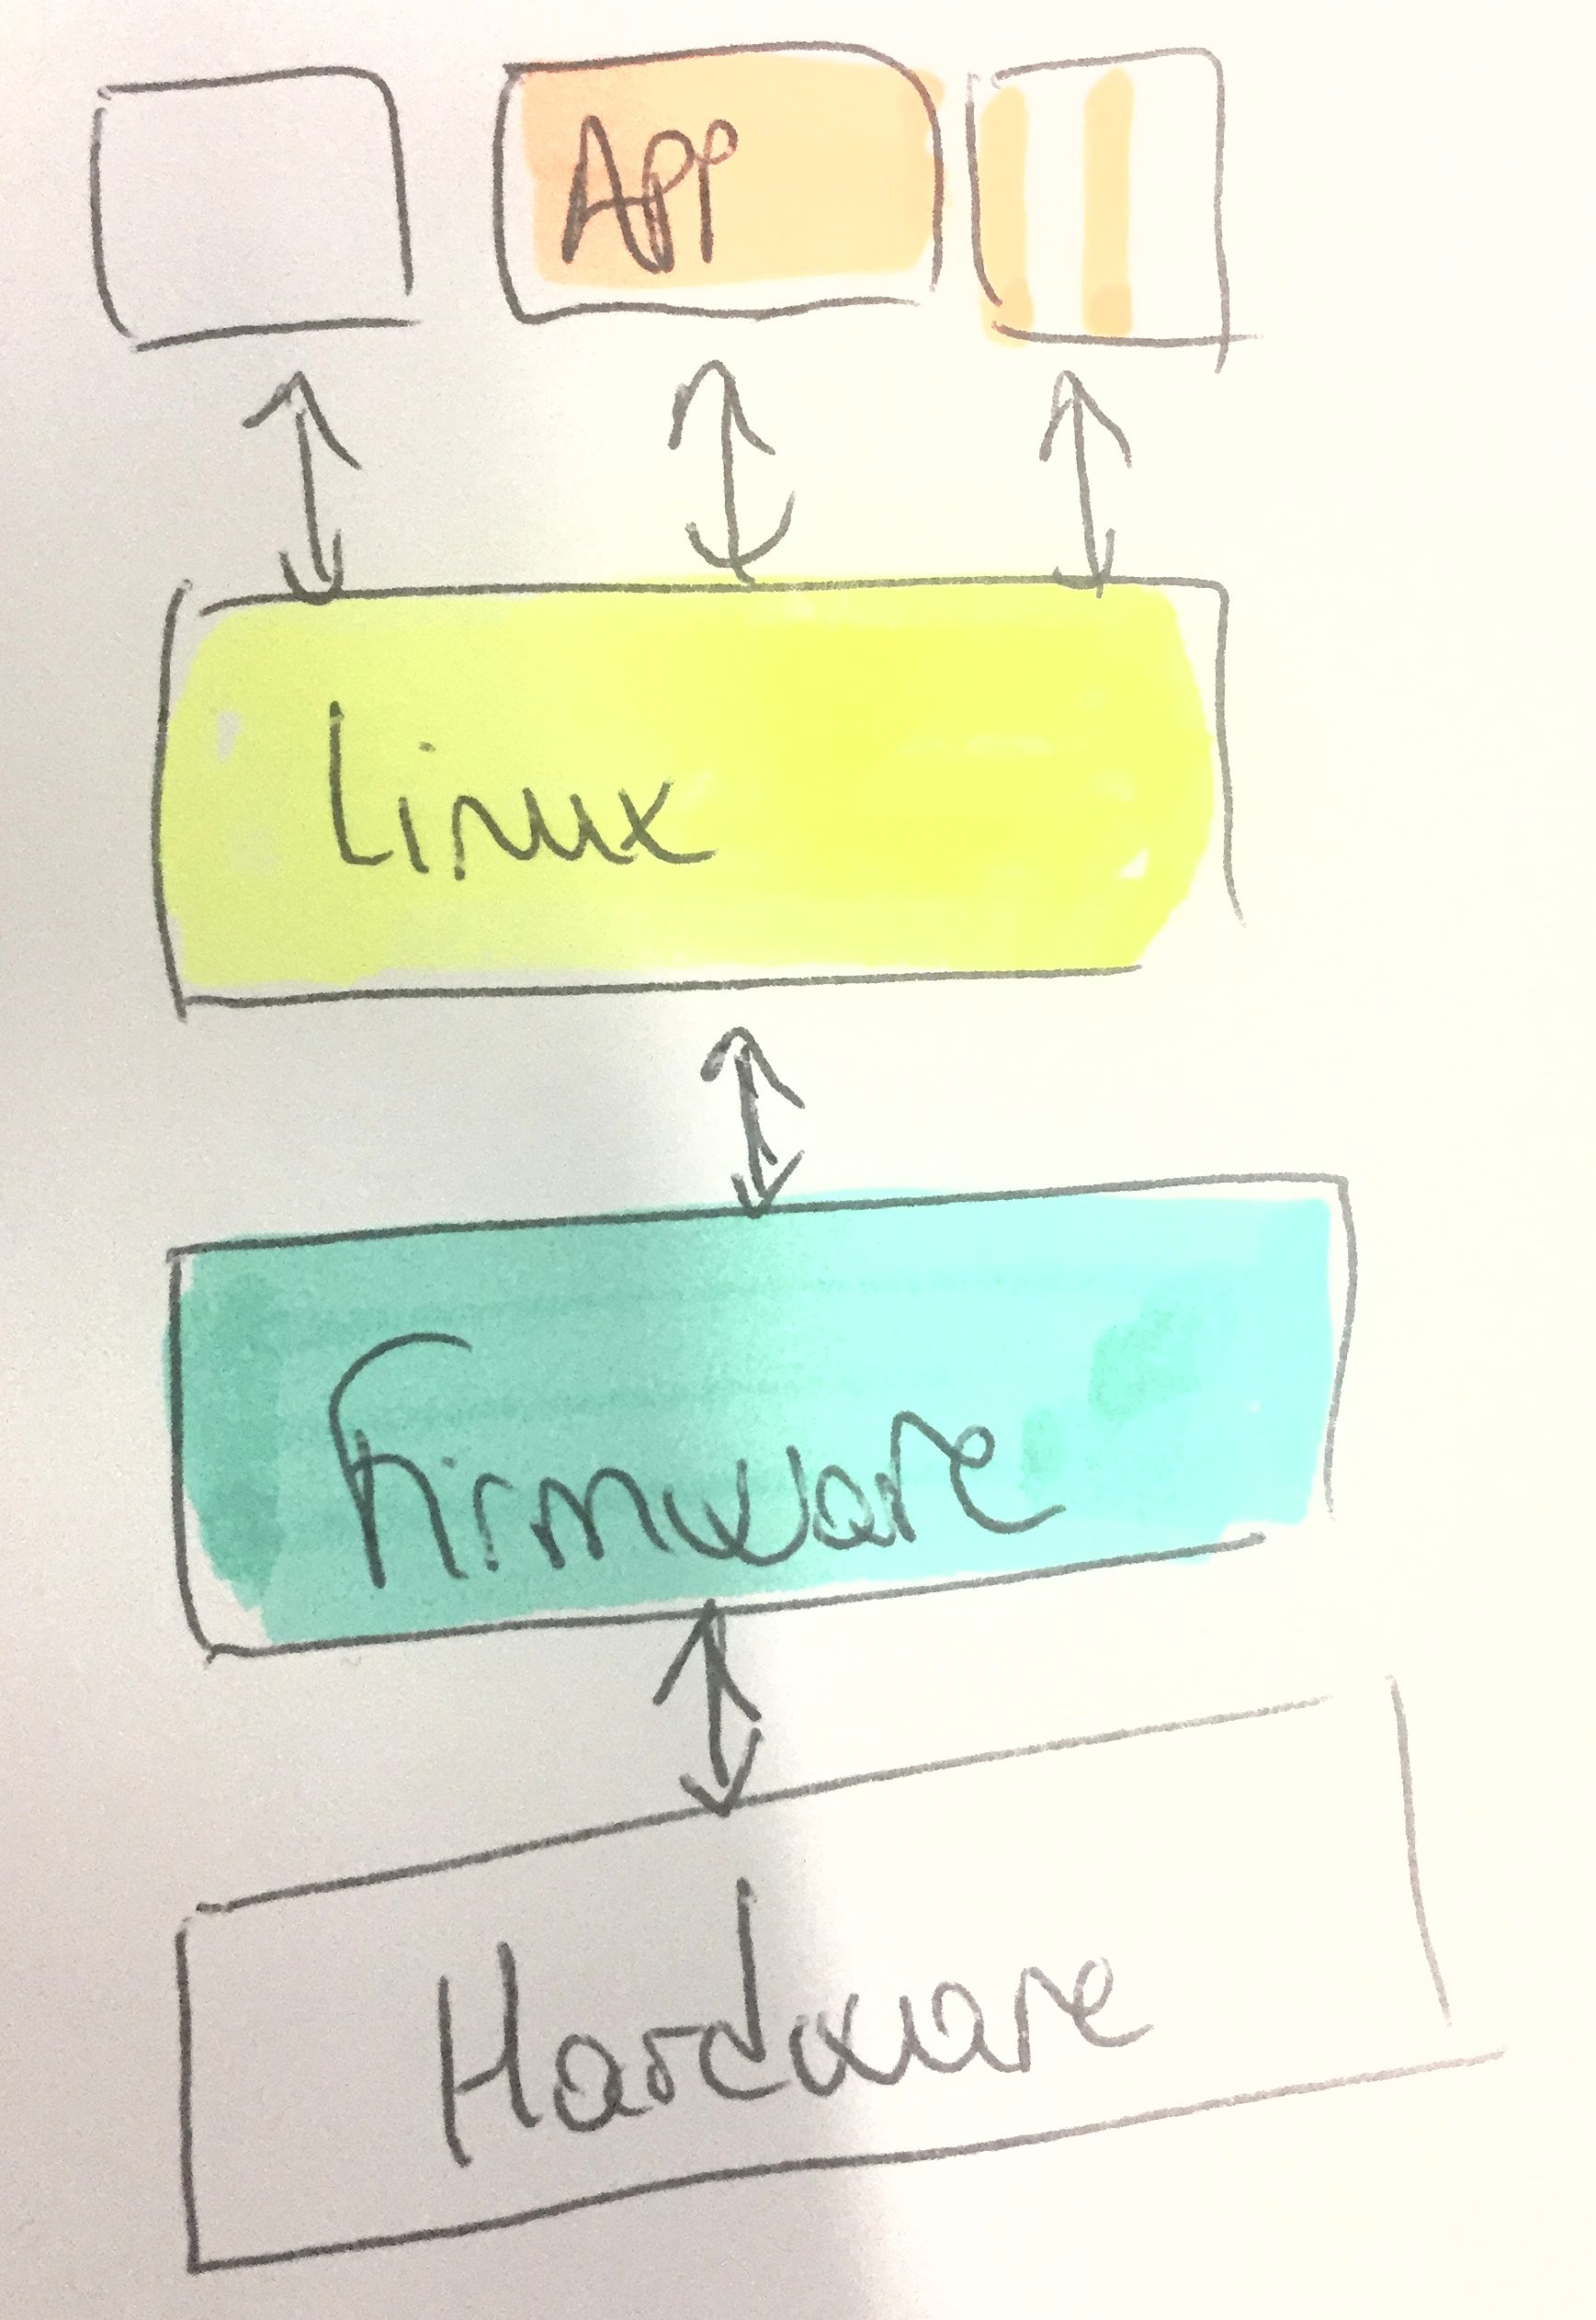
\includegraphics[width=0.3\textwidth]{Figures/computing-platform-1.jpg}
  \caption{Abstraction Layers of a Typical x86 Computing Platform}
  \label{fig:usecase:computing-platform-1}
\end{figure}

Figure\,\ref{fig:usecase:computing-platform-1} pictures the traditional
abstraction layers of a computing platform.
%
Each layer leverages the interface of its predecessor to expose a higher-level,
more constrained set of functionalities for its successors.
%
Thus, software developers who write end-user application do not need to handle
the complexity of x86, thanks to the principle of separation of concerns: while
the underlying operating system (and the firmware) handles the hardware specific
tasks, they can focus on application logic.
%
These interfaces are often standardize to some extend, which allows
interoperability.
%
This is useful because the market is characterized by a large diversity of
products for each layers.

Each layer is more privileged than its successors:
%
the hardware architecture executes the software stack;
%
the firmware has the mean to interrupt the execution of the other software
components;
%
the operating system loads in memory and manages the applications the user can
interact with.

\subsection{Hidden Hardware Architecture Complexity}

\begin{figure}
  \centering
  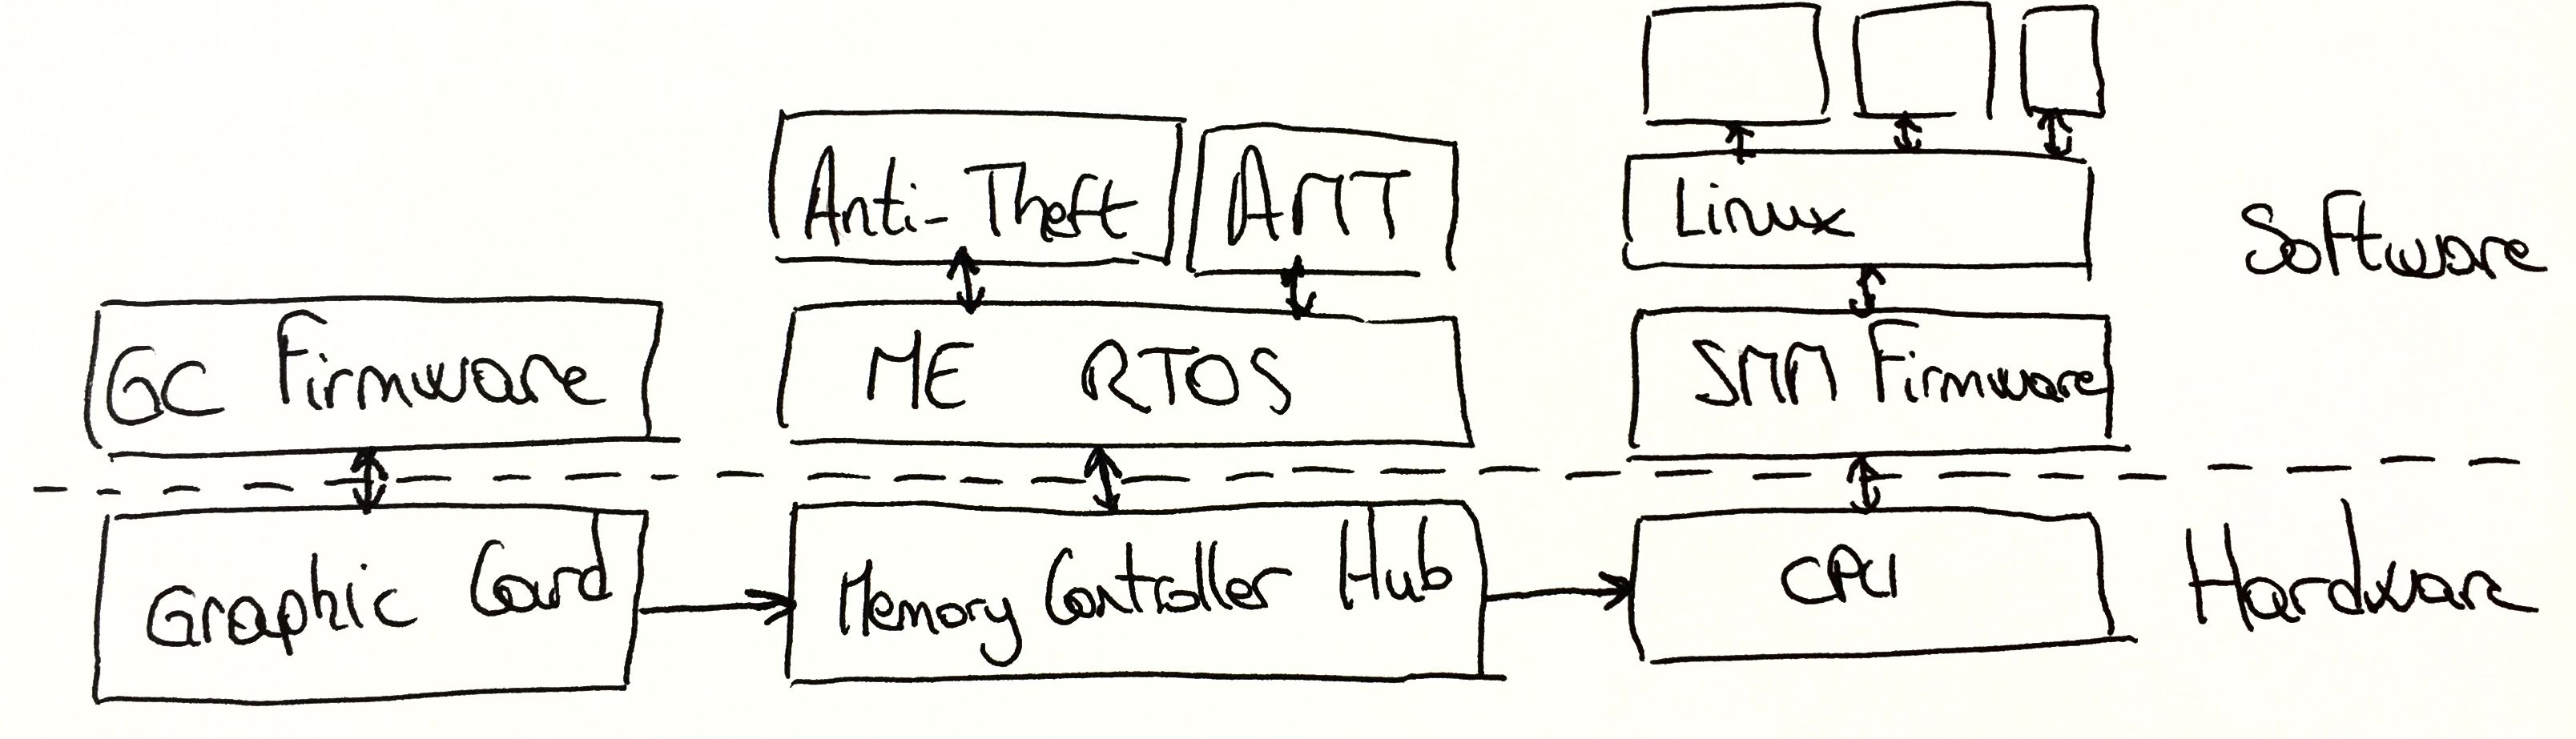
\includegraphics[width=0.8\textwidth]{Figures/intro-computing-platform.jpg}
  \caption{Hidden Hardware Architecture Complexity}
  \label{fig:usecase:computing-platform-2}
\end{figure}

One drawback of Figure\,\ref{fig:usecase:computing-platform-1} is to hide the
complexity of the \emph{Hardware} layer.
%
Far from a homogeneous block, a typical hardware architecture comprises dozens
of hardware components whose nature and purpose are very different.
%
It is not possible to reason about HSE mechanisms without taking this reality
into account.

Figure\,\ref{fig:usecase:computing-platform-2} partially highlights this, by
making explicit several hardware components involved in memory accesses: the
cache, the memory controller, a DRAM controller or potentially a graphic card.
%
Most of them run dedicated software stacks, concurrently with the ``main''
software stack pictured in Figure\,\ref{fig:usecase:computing-platform-1}.
%
Although these concurrent software stacks are not the main subject of this
thesis, they are worth mentioning, as they can have dramatic consequences from a
security perspective.
%
We cite two example to motivate this claim.
%
First, L. Duflot \emph{et al.} have been able to take control of a network card,
because the piece of software responsible for processing network packets was
vulnerable.
%
This novel ---at the time--- kind of attacks poses several challenges, from a
security perspective.
%
Indeed, it is very hard, if not impossible, for the ``main'' software stack to
know whether the network card has been compromised or not.
%
The second example we want to detail is the Intel Management Engine, an
autonomous system which lives inside x86 processors since 2008.
%
The Management Engine is used by Intel to provide business services, such as
out-of-band administration management or trusted computing technologies
emulation.
%
To enable these features, the Management Engine requires very important
privileges, and is \emph{de facto} the most privileged execution environment of
a x86 computing platform.
%
Recent vulnerabilities have shown this is not without consequences when the
Management Engine's software stack is compromised.

Apart from these potential software implementation issue within hidden software
stacks, Figure\,\ref{fig:usecase:computing-platform-2} highlights the complexity
of a typical hardware architecture.
%
This complexity easily explains the architectural attacks that have been
disclosed during the past decade.

\subsection{Software Isolation}

\begin{figure}
  \centering
  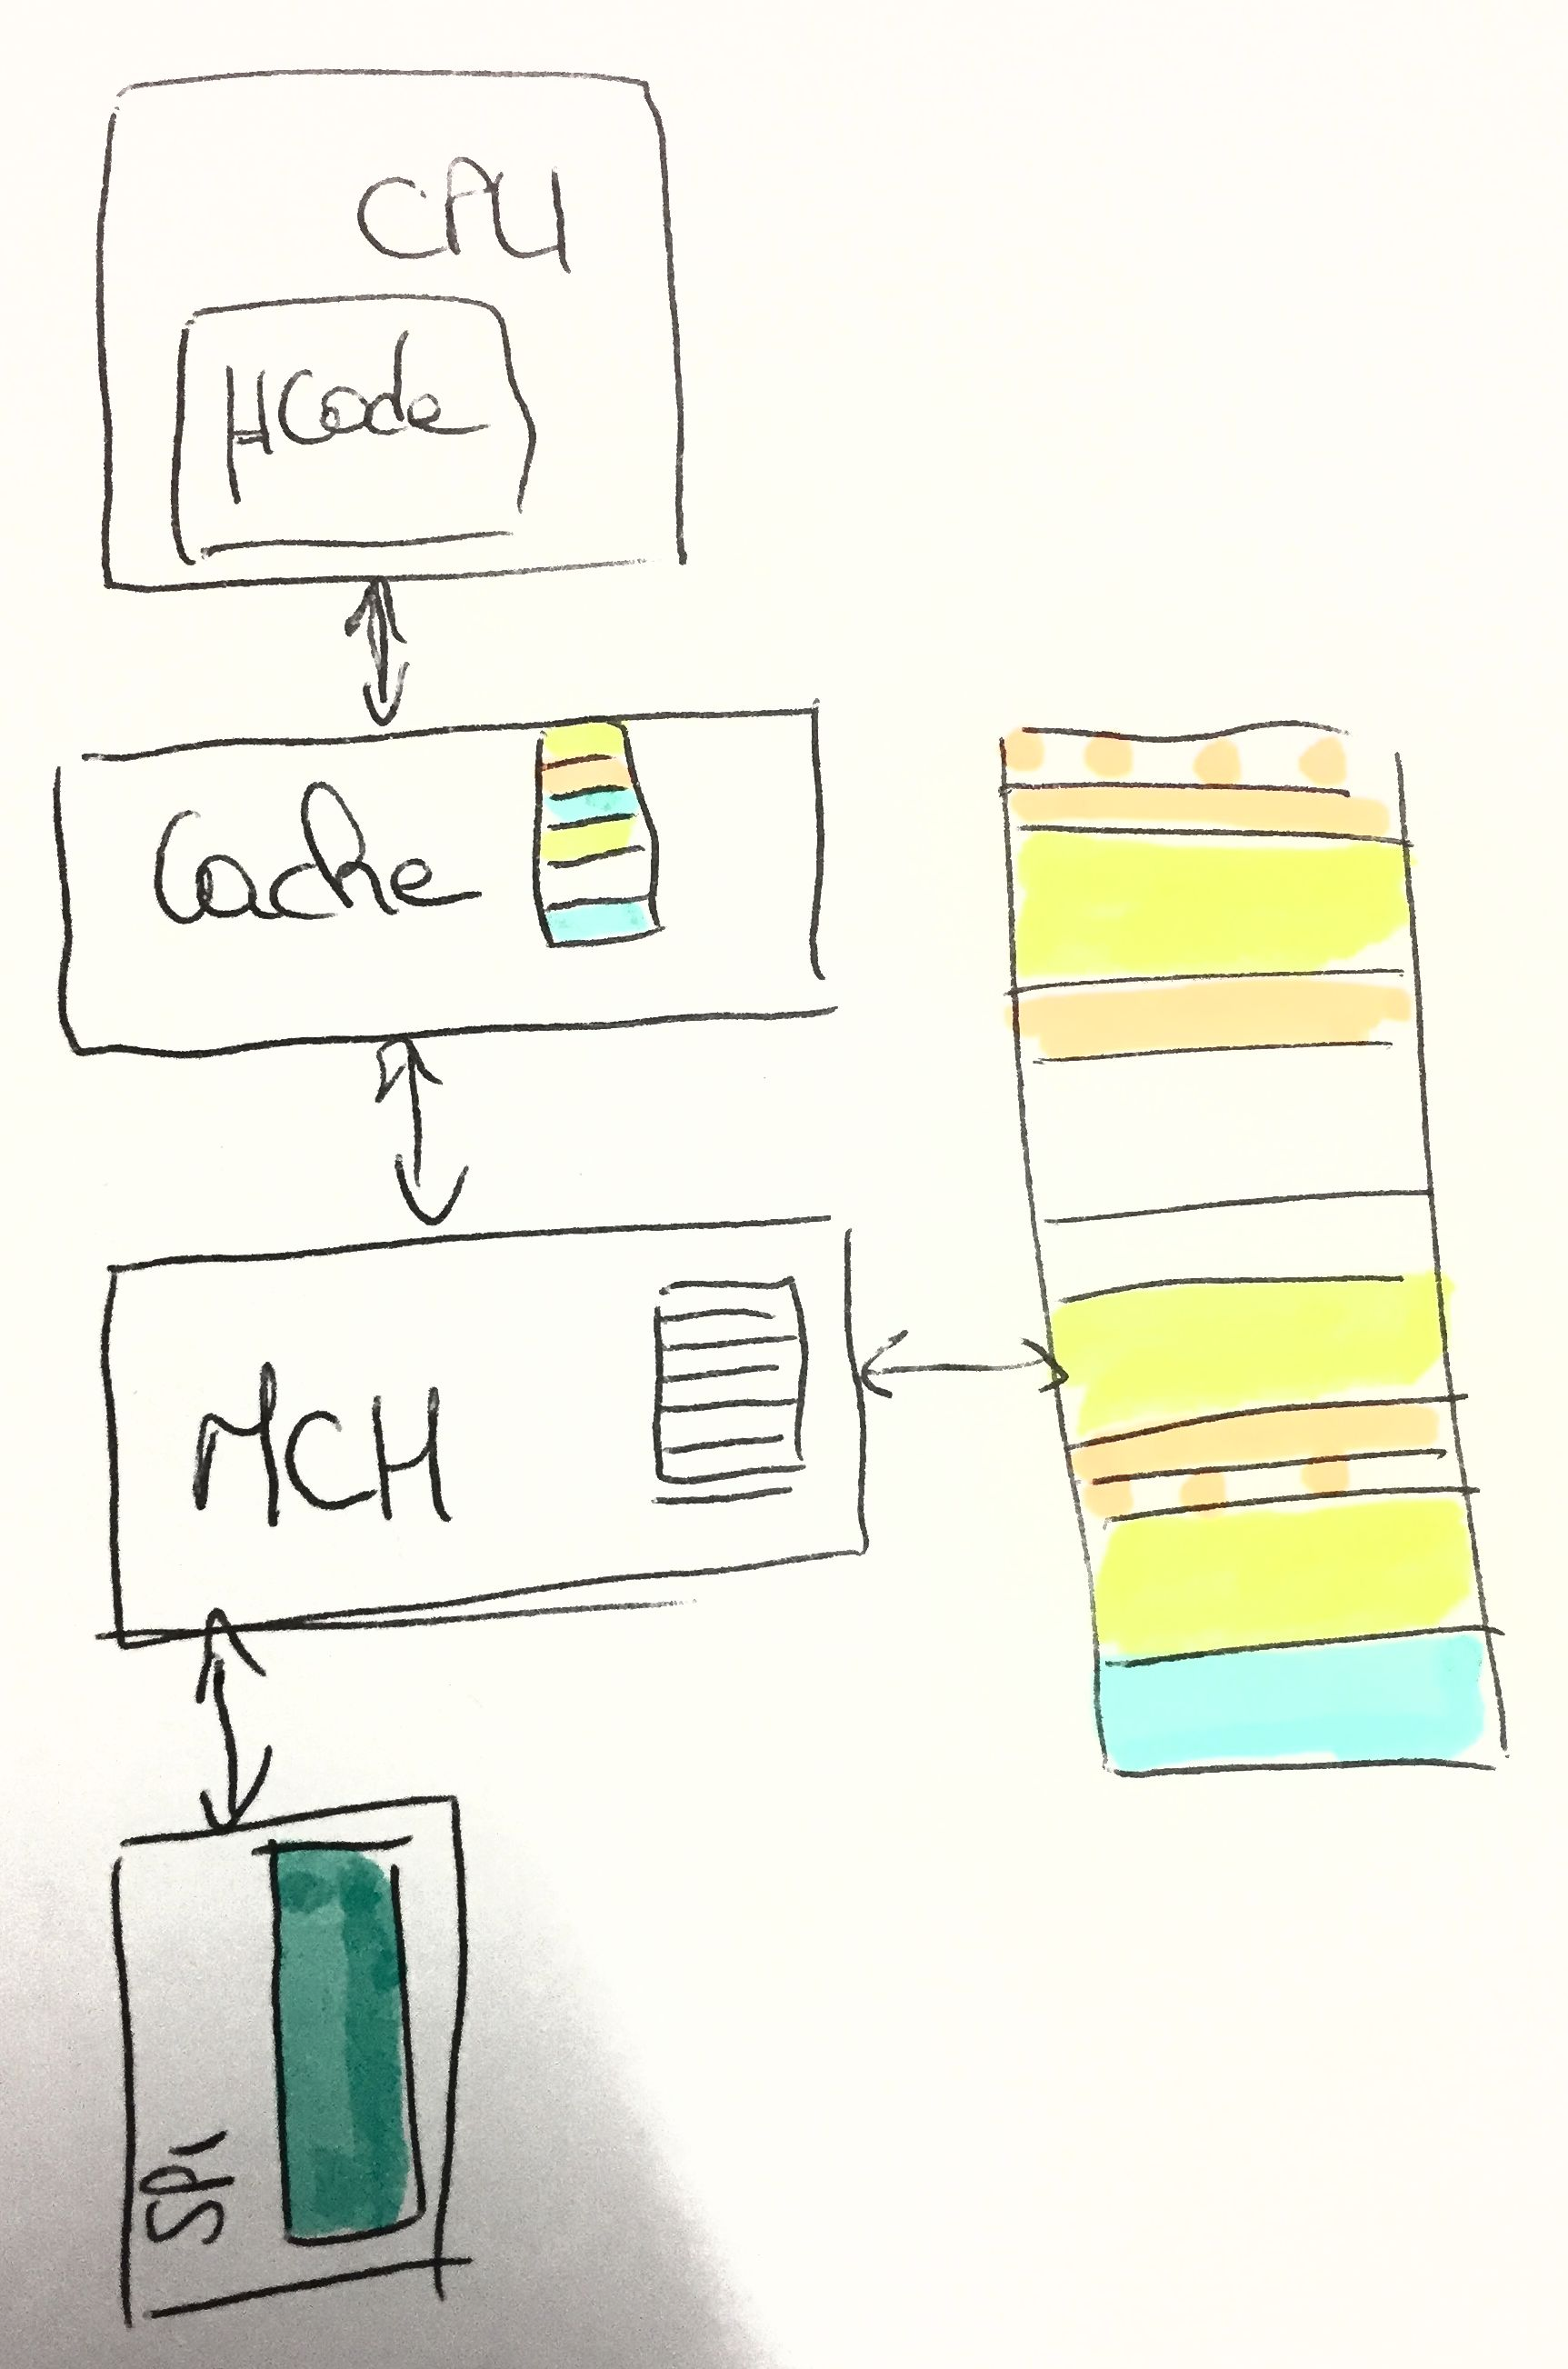
\includegraphics[width=0.3\textwidth]{Figures/computing-platform-3.jpg}
  \caption{Abstraction Layers of a Typical x86 Computing Platform}
  \label{fig:usecase:computing-platform-3}
\end{figure}

Software components mostly manipulate data stored in ``memory'', and they see
this memory as a continuous array.
%
In reality, it is scattered among many different, sometimes redundant locations.
%
This is partly because the x86 architecture heavily relies on \emph{memory
  mapping} mechanisms.
%
For each memory access, several hardware components might be involved: the MMU,
the cache, the memory controller, the DRAM controller, the peripherals, and so
on.

The code of the software components which form the software stack are also
stored within the memory, as pictured by
Figure\,\ref{fig:usecase:computing-platform-3}.
%
When the CPU wants to execute the next instruction of a given software
components code, it fetches it from memory.
%
For the result of this memory fetch to be what the software developer is
expecting, the memory layout has to be carefully configured.
%
This is harder than one might expect.
%
This makes \emph{isolation} a key security property.
%
In the context of this thesis, we say one component $A$ is said isolated from a
second component $B$ when $B$ cannot tamper with $A$'s functioning otherwise
than through its interface.
%
Thus, an operating system should be isolated from end users applications, to
prevent the latter to grant themselves abusive rights.
%
The opposite is not necessarily true, and it is even a common practice for
operating system to tamper with applications code (\emph{e.g.} address space
layout randomization, dynamic libraries).

Isolation should not been confused with code integrity, as it might be possible
for an attacker to tamper with the execution of a given software component
without modifying its code in memory.
%
To that end, they might for instance rely on a memory mapping mechanism.


\section{BIOS}
\label{sec:usecase:firmware}

To illustrate these threats, we focus on the \emph{Firmware} layer of the
computing platform.
%
We first explain the role played by the computer firmware at runtime, after the
boot sequence.
%
We then describe which HSE mechanisms it implements to stay isolated from the
rest of the software stack.
%
Finally, we show how these HSE mechanisms have been defeated by attackers over
time.

\subsection{BIOS Purposes}

In the context of this thesis, we call \emph{Firmware} a piece of software
provided by a hardware vendor and indispensable to ensure the computer correctly
works.
%
Many hardware components comes with their dedicated firmware, \emph{e.g.} the
graphic card, the network card, etc.
%
In addition, hardware vendors provide a particular form firmware tied to the
hardware architecture as a whole, better known as the \emph{Basic Input/Output
  System} (BIOS). % or the \emph{Unified Extensible Firmware Interface} (UEFI).

The main objective of the BIOS is to carry on the initialization of the hardware
architecture.
%
This initialization process is commonly called the boot sequence.
%
One the boot sequence is completed, the BIOS selects a system software, like an
operating system.
%
To do so, it loads the system software code into memory, then starts its
execution.
%
Once this is done, the system software controls the main CPU, and the rest of
the hardware architecture.

The BIOS often exposes a set of so-called runtime services, but nothing obliges
the system software to use them.
%
For this reason, people tend to think BIOS role ends with the boot sequence.
%
This is not true.
%
Indeed, the BIOS continues to actively participate to the well functioning of a
computer, even after it gives the control flow to the system software.
%
Its main task is to take care of hardware events specific to the particular
hardware architecture it is tied to.
%
Sometimes, it also emulates a hardware feature, in a transparent manner from the
point of view of the system software.  \thomasrk[inline]{Do we have an example?}
%
Last, but not least, it manages its own update.
%
That is, the system software is not able to modify the BIOS code, as stored in
the SPI Flash, by itself.
%
Instead, it can only submit an update to the BIOS, and the latter alone decides
if this update can be applied.
%
This prevent the dangerous scenario where an attacker is able to take control of
the system software, and then modify the BIOS.

Translated in terms of security properties, this means two things:
%
\begin{inparaenum}[(1)]
\item the BIOS shall be properly isolated from the other software components,
  and
  %
\item the SPI Flash which contains the BIOS code shall be integrity-protected,
  so that only the BIOS can modify it.
\end{inparaenum}
%
This should not be a surprise for the attentive readers: these two security
properties are enforced by two HSE mechanisms implemented by the BIOS.

\subsection{BIOS Isolation}

The BIOS Isolation at runtime is enforced thanks to the System Management Mode
(SMM) of x86 CPUs.
%
Intel describes it as follows (the emphasis is ours, and does not exist in the
original document):

\begin{quote}
  SMM is a special-purpose operating mode provided for handling system-wide
  functions like power management, system hardware control, or proprietary
  OEM-designed code.
  %
  It is intended for use only by system firmware, not b applications software or
  general-purpose systems software.
  %
  \textbf{The main benefit of SMM is that it offers a distinct and easily
    isolated processor environment that operates transparently to the operating
    system or executive and software applications.}
\end{quote}

To handle several level of privileges, Intel CPU provides several execution
modes.
%
An execution mode can be roughly assimilated to a set of hardware capabilities.
%
Hence, in a given execution mode, a CPU may refuse to execute certain assembly
instructions.
%
As a consequence, the software component executed will not be able to leverage
the side-effects involved by the execution of these instructions, \emph{e.g.}
access to specific hardware registers (like the one related to paging).
%
The execution modes are not ''linear''.
%
On the contrary, they can be seen as a composition of several hardware features:
ring levels, virtualization technology, and finally SMM.
%
This means you can be in ring 0, while in hypervisor mode, while in SMM, for
instance.

\paragraph{System Management Mode}
%
The main objective of the SMM, as stated by the Intel Developer Manual, is to
provide an `isolated processor environment'', dedicated to ``system firmware'',
and that should ``operate transparently to the operating system''.
%
To provide these features, SMM relies on two things: the SMRAM and the System
Management Interrupt (SMI)

The SMRAM is a special memory region within the DRAM, dedicated to the SMM.
%
It is supposed to contain the BIOS code, and its private data;
%
as a consequence, it should not be accessible to a CPU which is not in SMM.
%
The exact location and size of the SMRAM is architecture dependent.
%
To locate it, the CPU has a register named \texttt{SMBASE}, to be configured by
the BIOS during the boot sequence.
%
As its name implies, the \texttt{SMBASE} value should point to the base of the
SMRAM.
%
It is then up to the BIOS developer to appropriately write its so-called SMM
code (that is, the code supposedly executed in SMM during runtime) knowing the
limitation of the SMRAM of the targeted architecture.

The SMI is a hardware interrupt which makes the CPU enters SMM.
%
More precisely, when a CPU receives a SMI, it saves its current state
(\emph{e.g.} registers, execution mode, etc.), either in the SMRAM or, for most
recent versions, in dedicated register of the CPU.
%
Once this preliminary step is done, the CPU reconfigures itself;
%
in particular, it sets its program counter register, that is, the register which
indicates from which address to fetch the next instruction it shall execute, to
$\texttt{SMBASE} + 0x8000$\thomasrk{À vérifier.}.
%
From this point, the CPU is in SMM and starts to execute what should be the SMM
code.
%
Once the SMM code has performed the task it has been requested for, the
\texttt{rsm} instruction can be used.
%
The instruction, which can be used only in SMM, tells the CPU to restore its
previous state.
%
This way, the execution of the pieces of software previously halted by the SMI
can resume.
%
From the system point of view, it is like if nothing has happened.

\section{HSE}
\label{sec:usecase:hse}

The combination of the SMRAM and the SMI explains why the SMM is often
introduced as the ``most privileged execution mode'' of a x86 CPU.
%
In a nutshell, the SMM code can do all the thing the system software does,
including arbitrary memory locations which belongs to that system software, but
the system software cannot modify the SMRAM content.
%
In addition, the SMI is not a maskable interrupt, so the system software cannot
prevent the execution of the SMM code.
%
In other words, both the integrity of the SMRAM and the availability of the SMI
are the foundation of the SMM security.
%
Because they have been both defeated at repeated occasions, this makes the SMM
particularly interesting to illustrate the concept of architectural attacks.

\paragraph{SMRAM Cache Poisoning Attack}
%
From the beginning, the integrity of the SMRAM has been enforced by the Memory
Controller of the x86 architecture, whether it is a dedicated hardware component
(northbridge), or more recently a part of the CPU.
%
The Memory Controller main purpose it to act as a proxy for the CPU memory
accesses.
%
It receives the CPU memory accesses, and dispatches them among the different
hardware components which expose memory.

The Memory Controller exposes a configuration register called the
\texttt{SMRAMC}, whose purpose is to configure the access control configuration
of the SMRAM.
%
At the beginning of the boot sequence, the SMRAM is said to be opened, which
means it can be access by the CPU whether it is in SMM or not.
%
This allows the BIOS to load the SMM code inside the SMRAM, as the CPU is not
itself in SMM at the beginning of the boot sequence.
%
Once the loading is done, the BIOS can ``close'' the SMRAM, meaning only a CPU
in SMM can access to the SMRAM.
%
It can also lock the SMRAMC, to prevent further piece of software (say, a
malicious or exploited system software) to open the SMRAM in order to tamper
with its content.

Between 1986\thomasrk{Verify the date}, when the SMM has first been introduced,
and 2009, it was believed that the \texttt{SMRAMC} register enough was
sufficient to ensure the integrity of the SMRAM.
%
Loic Duflot \emph{et al.}\,\cite{duflot2009smram} and Rafal Wojtczuk \emph{et
  al.}\,\cite{wojtczuk2009smram} have independently shown this belief was
misplaced, thanks to the so-called \emph{SMRAM Cache Poisoning Attack}.
%
In addition to the evocative name, Figure\,\ref{todofig} highlights the
vulnerability concept.
%
To increase performance, the CPU uses a cache of its memory accesses.
%
That is, when it reads memory, it stores the result of this access within a
cache.
%
Then, when it has to read at the same location again, it gets the result from
the cache directly, whose access time is way lower than regular DRAM.
%
A similar scheme applies to write accesses.

As a consequence, regarding a CPU configuration, copies of the SMRAM content may
be found in the cache.
%
These copies were not protected by the Memory Controller, meaning the system
software could tamper with them, even while not in SMM.
%
This attack is a perfect illustration of an architectural attack:
%
both the Memory Controller and the Cache work as expected.
%
The first one prevent an authorized access by a CPU not in SMM;
%
The second one keeps copies of successful accesses to decrease latency due to
memory accesses.
%
However, once put together, they paves the road toward a successful tampering of
the SMRAM by a system software.

The solution implemented by Intel to prevent further exploitation of this
vulnerability was to modify the behavior of the Cache, when the memory accesses
target the SMRAM;
%
and because the SMRAM size and location remain specific to each architecture,
this means it requires an additional step of configuration to tell the cache
where the SMRAM is.

What is interesting about the SMRAM Cache Poisoning is that another x86
vulnerability\,\cite{domas2015sinkhole} has been since disclosed.
%
It also allows to trick a CPU in SMM to execute arbitrary instructions, but
leaves the content of the SMRAM in DRAM untouched.
%
In this case, it leverages the fact that the configuration registers of the
APIC\,\footnote{\emph{Advanced Programmable Interrupt Controller}.}, a component
of the CPU, can be mapped in memory.
%
An attacker can use them to mask the real content of the SMRAM, even to a CPU in
SMM.
%
Again, the complexity implied by the composition of several hardware components
can be used in a harmful way.


\paragraph{SPI Flash Integrity}
%
The isolation provided by the SMM is not an end in itself.
%
In fact, it has become the basis upon which other HSE mechanisms have been
implemented.
%
One good example is the HSE mechanism responsible for the SPI Flash access
control.
%
In this example, the trusted software component is the SMM code.
%
The rest of the software stack, including the system software, is considered
untrusted.
%
The targeted security property is the integrity of the SPI Flash.
%
More precisely, only the SMM code should be capable of overwriting the content
of the SPI Flash, which contains the BIOS code.
%
To enforce this security property, the HSE mechanism relies on the
\texttt{FNCTL} \thomasrk{Trouver le bon nom et mettre une ref.} register,
exposed by the Platform Controller Hub.
%
Once configured correctly, the SPI Flash is considered ``locked'', meaning it is
not possible even for the SMM code to issue a successful write access which
targets its content.
%
The SPI Flash can be unlocked, but when the system software tries, the PCH fires
a SMI.
%
As a consequence, the CPU saves its current state, and starts executing the SMM
code.

What comes next depends on the SMM code, and how it is implemented.
%
It is executed in a situation where the SPI Flash is unlocked, so it can
perform, if it makes sense, the write access intended by the system software on
its behalf.
%
On typical workflow is for the system software to load the BIOS update in
memory, and for the SMM code to verify whether this update is correctly signed
by the vendor.
%
In any case, it is the responsibility of the SMM code to lock again the SPI
Flash before it uses the \texttt{rsm} instruction to leave SMM.
%
Similarly to the \texttt{SMRAMC} register and the isolation it promises, the
\texttt{FNCTL} register has been defeated at least twice.

\paragraph{SENTER Sandman}
%
In 2015, Xeno Kovah \emph{et al.} have shown it was possible to leverage the
Intel TXT technology to circumvent the SPI Flash write
protection\,\cite{kovah2015senter}.
%
By default, a system software has to trust the BIOS.
%
Nowadays, most BIOS implementations are made of millions of lines of code, which
are provided by many different industrial partners of the vendor.
%
As a consequence, the attack surface is consequent.
%
Intel TXT is a recent feature of some x86 CPU, whose aim is to reduce the
Trusted Computing Base (TCB) of a system software, by removing most of the BIOS
from it.
%
With Intel TXT, a hypervisor can start its execution in an isolated execution
environment.
%
From this perspective, it was coherent for TXT to mask incoming SMIs, this
indeed reduce the size of the TCB, by excluding the SMM code.
%
Unfortunately, in this case, it has the important consequence of leaving the SPI
Flash content unprotected.

\paragraph{Speed Racer}
%
There is at least another attack that defeated the \texttt{FNCTL} register
purpose.
%
In 2015, Corey Kallenberg \emph{et al.} have shown that the scenario detailed
previously, where unlocking the SPI Flash fires a SMI which forces the CPU to
execute the SMM code, suffers from a race condition in presence of a second
CPU\,\cite{kallenberg2015racecondition}.
%
When a SMI is fired, all the x86 CPU of the platform will eventually enter in
SMM.
%
On the contrary, the SPI Flash is unlocked as soon as the \texttt{FNCTL}
register is modified.
%
To prevent this race condition, Intel has added a new feature to its PCH, and
exposed by the \texttt{FNCTL} register.
%
Once activated, this new feature ensures the SPI Flash stays locked as long as
one CPU is not in SMM.

\section{Conclusion}
\label{sec:usecase:conclusion}

Due to the complexity of computing platform, in particular from a hardware point
of view, implementing a correct HSE mechanism is challenging.
%
We chose to focus on HSE mechanisms implemented by the firmware, because it has
been well studied and there are several illustrative example of architectural
attacks.
%
In particular, in this chapter, we explained how three of them work.
